
\documentclass{Configuration_Files/PoliMi3i_thesis}

%------------------------------------------------------------------------------
%	REQUIRED PACKAGES AND  CONFIGURATIONS
%------------------------------------------------------------------------------

% CONFIGURATIONS
\usepackage{parskip} % For paragraph layout
\usepackage{setspace} % For using single or double spacing
\usepackage{emptypage} % To insert empty pages
\usepackage{multicol} % To write in multiple columns (executive summary)
\setlength\columnsep{15pt} % Column separation in executive summary
\setlength\parindent{0pt} % Indentation
\raggedbottom  

% PACKAGES FOR TITLES
\usepackage{titlesec}
% \titlespacing{\section}{left spacing}{before spacing}{after spacing}
\titlespacing{\section}{0pt}{3.3ex}{2ex}
\titlespacing{\subsection}{0pt}{3.3ex}{1.65ex}
\titlespacing{\subsubsection}{0pt}{3.3ex}{1ex}
\usepackage{color}

% PACKAGES FOR LANGUAGE AND FONT

\usepackage[utf8]{inputenc} % UTF8 encoding
\usepackage[T1]{fontenc} % Font encoding
\usepackage[11pt]{moresize} % Big fonts

% PACKAGES FOR IMAGES
\usepackage{graphicx}
\usepackage{transparent} % Enables transparent images
\usepackage{eso-pic} % For the background picture on the title page
\usepackage{subfig} % Numbered and caption subfigures using \subfloat.
\usepackage{tikz} % A package for high-quality hand-made figures.
\usetikzlibrary{}
\graphicspath{{./Images/}} % Directory of the images
\usepackage{caption} % Coloured captions
\usepackage{xcolor} % Coloured captions
\usepackage{amsthm,thmtools,xcolor} % Coloured "Theorem"
\usepackage{float}

% STANDARD MATH PACKAGES
\usepackage{amsmath}
\usepackage{amsthm}
\usepackage{amssymb}
\usepackage{amsfonts}
\usepackage{bm}
\usepackage[overload]{empheq} % For braced-style systems of equations.
\usepackage{fix-cm} % To override original LaTeX restrictions on sizes

% PACKAGES FOR TABLES
\usepackage{tabularx}
\usepackage{longtable} % Tables that can span several pages
\usepackage{colortbl}

% PACKAGES FOR ALGORITHMS (PSEUDO-CODE)
\usepackage{algorithm}
\usepackage{algorithmic}

% PACKAGES FOR REFERENCES & BIBLIOGRAPHY
\usepackage[colorlinks=true,linkcolor=black,anchorcolor=black,citecolor=black,filecolor=black,menucolor=black,runcolor=black,urlcolor=black]{hyperref} % Adds clickable links at references
\usepackage{cleveref}
\usepackage[square, numbers, sort&compress]{natbib} % Square brackets, citing references with numbers, citations sorted by appearance in the text and compressed
\bibliographystyle{abbrvnat} % You may use a different style adapted to your field

% OTHER PACKAGES
\usepackage{pdfpages} % To include a pdf file
\usepackage{afterpage}
\usepackage{lipsum} % DUMMY PACKAGE
\usepackage{fancyhdr} % For the headers
\fancyhf{}

% Input of configuration file. Do not change config.tex file unless you really know what you are doing. 
% Define blue color typical of polimi
\definecolor{bluepoli}{cmyk}{0.4,0.1,0,0.4}

% Custom theorem environments
\declaretheoremstyle[
  headfont=\color{bluepoli}\normalfont\bfseries,
  bodyfont=\color{black}\normalfont\itshape,
]{colored}

% Set-up caption colors
\captionsetup[figure]{labelfont={color=bluepoli}} % Set colour of the captions
\captionsetup[table]{labelfont={color=bluepoli}} % Set colour of the captions
\captionsetup[algorithm]{labelfont={color=bluepoli}} % Set colour of the captions

\theoremstyle{colored}
\newtheorem{theorem}{Theorem}[chapter]
\newtheorem{proposition}{Proposition}[chapter]

% Enhances the features of the standard "table" and "tabular" environments.
\newcommand\T{\rule{0pt}{2.6ex}}
\newcommand\B{\rule[-1.2ex]{0pt}{0pt}}

% Pseudo-code algorithm descriptions.
\newcounter{algsubstate}
\renewcommand{\thealgsubstate}{\alph{algsubstate}}
\newenvironment{algsubstates}
  {\setcounter{algsubstate}{0}%
   \renewcommand{\STATE}{%
     \stepcounter{algsubstate}%
     \Statex {\small\thealgsubstate:}\space}}
  {}

% New font size
\newcommand\numfontsize{\@setfontsize\Huge{200}{60}}

% Title format: chapter
\titleformat{\chapter}[hang]{
\fontsize{50}{20}\selectfont\bfseries\filright}{\textcolor{bluepoli} \thechapter\hsp\hspace{2mm}\textcolor{bluepoli}{|   }\hsp}{0pt}{\huge\bfseries \textcolor{bluepoli}
}

% Title format: section
\titleformat{\section}
{\color{bluepoli}\normalfont\Large\bfseries}
{\color{bluepoli}\thesection.}{1em}{}

% Title format: subsection
\titleformat{\subsection}
{\color{bluepoli}\normalfont\large\bfseries}
{\color{bluepoli}\thesubsection.}{1em}{}

% Title format: subsubsection
\titleformat{\subsubsection}
{\color{bluepoli}\normalfont\large\bfseries}
{\color{bluepoli}\thesubsubsection.}{1em}{}

% Shortening for setting no horizontal-spacing
\newcommand{\hsp}{\hspace{0pt}}

\makeatletter
% Renewcommand: cleardoublepage including the background pic
\renewcommand*\cleardoublepage{%
  \clearpage\if@twoside\ifodd\c@page\else
  \null
  \AddToShipoutPicture*{\BackgroundPic}
  \thispagestyle{empty}%
  \newpage
  \if@twocolumn\hbox{}\newpage\fi\fi\fi}
\makeatother

%For correctly numbering algorithms
\numberwithin{algorithm}{chapter}

%----------------------------------------------------------------------------
%	NEW COMMANDS DEFINED
%----------------------------------------------------------------------------

% EXAMPLES OF NEW COMMANDS
\newcommand{\bea}{\begin{eqnarray}} % Shortcut for equation arrays
\newcommand{\eea}{\end{eqnarray}}
\newcommand{\e}[1]{\times 10^{#1}}  % Powers of 10 notation

%----------------------------------------------------------------------------
%	ADD YOUR PACKAGES (be careful of package interaction)
%----------------------------------------------------------------------------
\definecolor{codegreen}{rgb}{0,0.6,0}
\definecolor{codegray}{rgb}{0.5,0.5,0.5}
\definecolor{codepurple}{rgb}{0.58,0,0.82}
\definecolor{backcolour}{rgb}{0.95,0.95,0.92}
\usepackage{color}   %May be necessary if you want to color links
\usepackage{hyperref}
\usepackage{graphicx}
\usepackage[utf8]{inputenc}
\usepackage{listings}
\usepackage{xcolor}
\hypersetup{
	colorlinks=true, %set true if you want colored links
	linktoc=all,     %set to all if you want both sections and subsections linked
	linkcolor=black,  %choose some color if you want links to stand out
	urlcolor=blue,
}
\lstdefinestyle{mystyle}{
	backgroundcolor=\color{backcolour},
	commentstyle=\color{codegreen},
	keywordstyle=\color{magenta},
	numberstyle=\tiny\color{codegray},
	stringstyle=\color{codepurple},
	basicstyle=\ttfamily\footnotesize,
	breakatwhitespace=false,
	breaklines=true,
	captionpos=b,
	keepspaces=true,
	numbers=left,
	numbersep=5pt,
	showspaces=false,
	showstringspaces=false,
	showtabs=false,
	tabsize=2
}

\lstset{style=mystyle}


%----------------------------------------------------------------------------
%	BEGIN OF YOUR DOCUMENT
%----------------------------------------------------------------------------

\begin{document}

\fancypagestyle{plain}{%
\fancyhf{} % Clear all header and footer fields
\fancyhead[RO,RE]{\thepage} %RO=right odd, RE=right even
\renewcommand{\headrulewidth}{0pt}
\renewcommand{\footrulewidth}{0pt}}

%----------------------------------------------------------------------------
%	TITLE PAGE
%----------------------------------------------------------------------------

\pagestyle{empty} % No page numbers
\frontmatter % Use roman page numbering style (i, ii, iii, iv...) for the preamble pages

\puttitle{
	title=Systems and Methods for Big and Unstructured Data Project,
	name1=Gabriele Ginestroni, % Author Name and Surname
	name2=Giacomo Gumiero,
	name3=Lorenzo Iovine,
	name4=Nicola Landini,
	name5=Francesco Leone,
	academicyear=2022-2023,
	groupnumber=10
} % These info will be put into your Title page

\startpreamble
\setcounter{page}{1} % Set page counter to 1

%----------------------------------------------------------------------------
%	LIST OF CONTENTS/FIGURES/TABLES/SYMBOLS
%----------------------------------------------------------------------------

% TABLE OF CONTENTS
\thispagestyle{empty}
\tableofcontents % Table of contents
\thispagestyle{empty}
\cleardoublepage

\addtocontents{toc}{\vspace{2em}} % Add a gap in the Contents, for aesthetics
\mainmatter % Begin numeric (1,2,3...) page numbering

\chapter{Introduction}
\label{ch:introduction}
In this chapter will be presented the problem specification and the hypothesis under which the database is implemented.

\section{Problem Specification}
This project aims to build a documental database that handles scientific articles contained in the DBLP bibliography.
The focus is on creating a database which allows efficient information retrieval from the publications citation network.
The main collections analyzed in the project are \emph{Author} and \emph{Publication} with all their attributes and related
objects like: \emph{Venue, FieldOfStudy, Chapter} and \emph{Image}.

\section{Assumptions}


\chapter{ER Diagram}
\label{ch:erd}
\begin{figure}[H]
	\centering
	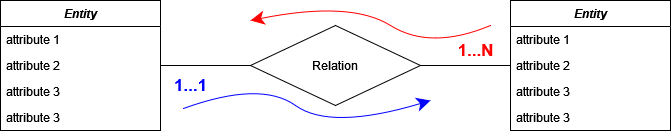
\includegraphics[width=0.6\textwidth]{legendaER.png}
	\caption{ER Diagram Organization}
	\label{fig:erleg}
\end{figure}
\bigskip
\begin{figure}[H]
	\centering
	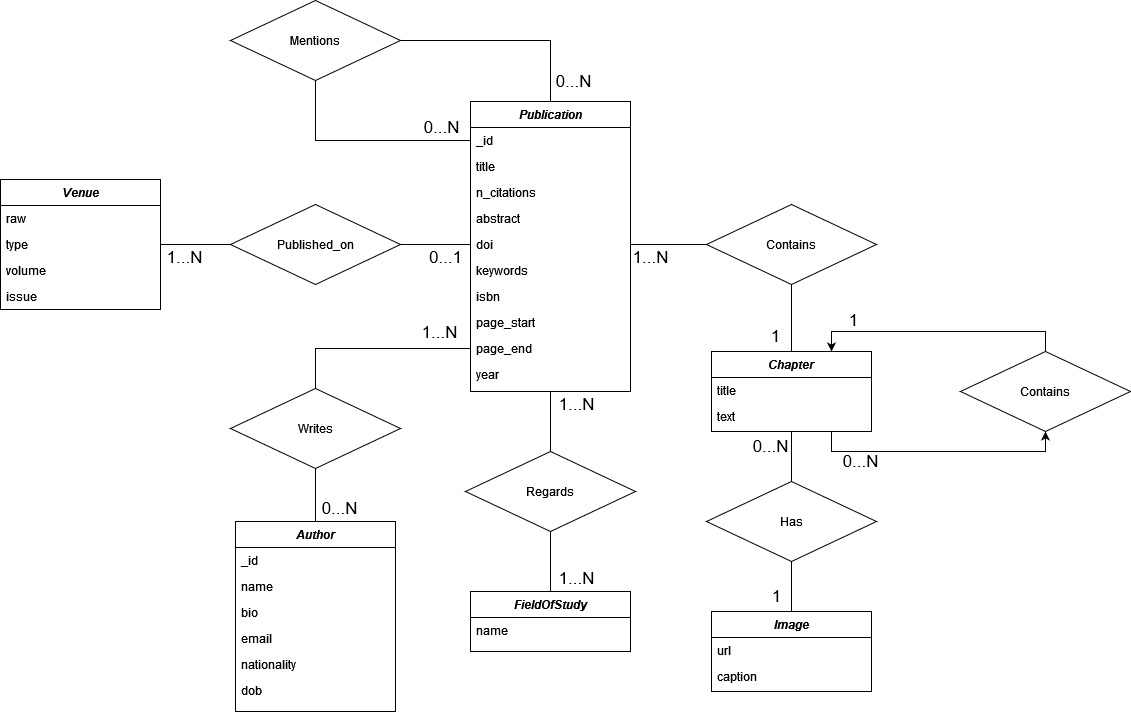
\includegraphics[width=1\textwidth]{ERDocDb.png}
	\caption{ER Diagram}
	\label{fig:er}
\end{figure}
\newpage

The Entity-Relationship model contains 6 main entities, that are related to each other through various relationships:
\begin{itemize}
	\item \textbf{Publication:} represents all the scientific articles. Its attributes are: \emph{\_id, title, n\_citations,
		abstract, doi, keywords, isbn, page\_start, page\_end, year} and its organization will be presented later
	\item \textbf{Author:} it is the one who contributed to a publication. Its attributes are: \emph{\_id, name, bio,
		email, nationality, dob (date of birth)}
	\item \textbf{Venue:} it is where a publication is published or presented. Its attributes are: \emph{raw, type,
		volume, issue}
	\item \textbf{FieldOfStudy:} this entity represents the subjects of the publication and its attribute is \emph{name}
	\item \textbf{Chapter:} it represents the chapter of a scientific articles. Its attributes are \emph{title, text}
	\item \textbf{Image:} it represents the image contained in a specific chapter of the publication. Its attributes are
		\emph{url, caption}
\end{itemize}

The ER diagram designed contains also the following relationships:
\begin{itemize}
	\item \textbf{Mentions:} is the relationship between a \emph{publication} and another \emph{publication} cited by the first one
	\item \textbf{Published\_on:} is the relationship between a \emph{publication} and its \emph{venue}
	\item \textbf{Writes:} is the relationship between \emph{author} and \emph{publication} which features the affiliation property
		We decided to design it with \verb |affiliation| as an attribute of the relationship, due to the fact that it belongs
		only to a pair of \emph{author} and \emph{publication} and it represents the institute where the author worked for the publication
	\item \textbf{Regards:} is the relationship between a \emph{publication} and its \emph{fields of study}
	\item \textbf{Contains:} is the relationship between \emph{publication} and its \emph{chapters} 
	\item \textbf{Composed\_by:} is the relationship between two \emph{chapters}. It represents the relationship created
		between a chapter and its sections, between a section and its subsection and so on. Note that we used a directed
		arrow in order to indicate that a section belongs only to a chapter, but a chapter could own more than one section.
	\item \textbf{Has:} is the relationship between \emph{chapter} and its \emph{images}
\end{itemize}



\chapter{Sample Dataset}
\label{ch:sample_dataset}


\chapter{Commands and Queries}
\label{ch:ceq}
\section{Commands}
We have identified the following \verb |INSERT| and \verb |UPDATE| commands to show the system basic functionalities.

\subsection{Insert an author in the system}
Assuming he is not present in the dataset, we used \verb |insertOne| to create a new instance of \emph{Author}.
\begin{lstlisting}
db.authors.insertOne([
	name: "Emanuele Della Valle",
	orcid: "0000-0002-5176-5885",
	articles:[
		{}
	]
])
\end{lstlisting}




\end{document}
